% -*- root: ../../main.tex -*
%!TEX root = ../../main.tex
% vim:textwidth=80 fo=cqt conceallevel=0


Varying the  number of electrochemical  layers stacked  within a pouch  cell has
contrasting effects  on its energy  storage and power handling  capabilities. In
this section,  a high-level  intuitive explanation of  this phenomenon  is first
offered, before  delving into  a detailed  presentation of  this effect  and its
implications for a specific  example cell in \cref{sec:energypowertradeoffdemo}.
Interwoven into the  narrative is a set of simplifying  assumptions made by this
thesis  author, which  sets the  broader  context within  which a  computational
framework for  determining the optimum  number of  layers for a  specific target
design shall be formalised and presented in \cref{sec:layeroptframework}.

\subsection{Preliminary assumptions}\label{subsec:layeroptassumptions}

To  obtain a  balanced  loading of  both electrodes  and  to avoid  asymmetrical
exhaustion  of lithium  from  one  of the  electrodes  during  operation, it  is
desirable to carefully calculate the  volume of electrochemical active materials
to be accommodated  within the cell. This concept is  well-known and is commonly
discussed  in  standard  textbooks in  the  field  such  as  those by  Rahn  and
Wang~\cite{Rahn2013} wherein  example calculations are presented  for non-porous
electrodes.

In  the  case  of  lithium  ion   cells  with  porous  electrodes,  the  concept
of  electrode-balancing  involves an  additional  variable  \viz{} the  porosity
of  the  active materials.  The  role  of  porosity  and its  corollaries  \ie{}
the  material  volume  fraction  and  filler/binder  fraction  is  discussed  in
\cref{subsec:spmp2dparametrisation}.  In this  work,  a  major assumption  about
material porosities  (and hence active-material/filler volume  fraction) is that
they are held constant. The rationale behind using this simplified assumption is
as follows.

This  author  visualises  the  integration  of  cell-level  design  optimisation
(through  an optimal  layer  selection procedure)  into  the overall  drivetrain
design  by the  \emph{cell manufacturer}  before  a custom  design is  delivered
to  vehicle/system  integrators.   Cell  manufacturers,  especially  small-scale
manufacturers do not necessarily  synthesize each electrochemical component, but
instead may opt  to source certain raw-materials from  an upstream supply-chain.
From  a  manufacturing  viewpoint,  the  porosity  of  the  electrode  materials
is  governed  by  the  extent  of  calendaring  of  the  electrode  reel.  Using
pre-calendered electrode materials or sourcing  large volumes of electrode reels
with a fixed extent of calendaring can help to keep costs low. In the absence of
a concrete  insight into  the procuring process,  this represents  a preliminary
justification of the author's assumption about constant porosities.

From a technical  viewpoint, there exists another redeeming  argument to support
the constant  porosity assumption. Keeping material  porosities constant enables
to eliminate a  degree of freedom in the design  optimisation, thereby narrowing
the dimensionality of  the search space. To the best  of the author's knowledge,
there has not  yet been any published work tackling  layer optimisation of pouch
cells.  Building an  initial  infrastructure \viz{}  a computational  framework,
based upon this constant porosity approximation shall provide a solid foundation
to build upon and extend for such  real-life use-cases. The author views this as
a vanguard research  into cell engineering and therefore places  a high value in
obtaining ballpark  estimates of  an optimal layer  count, albeit  with constant
porosities. Nevertheless,  the influence of  varying the material  porosities on
the cell's  performance is to be  quantified. Therefore, prior to  adopting this
model-based  methodology  for production  yields  at  scale, a  fully-integrated
design optimisation process  with variable porosities have to  be accounted for.
In this work, the author restricts the study to constant porosity values, whilst
acknowledging  variable  porosity designs  as  an  important aspect  for  future
studies.

At  a  system level,  the  efficiency  of the  drivetrain  is  considered to  be
constant. The  drivetrain of  an electric  vehicle consists of  a whole  host of
electrical as well as mechanical  components such as power electronics, electric
motors and  transmission. The efficiencies  of each  of these components  have a
cascading effect  on the overall  drivetrain efficiency. The efficiency  of each
component  is strongly  dependent upon  the operating  point. For  instance, the
efficiency of  an electric  motor is  a function of  its torque-speed  curve. In
practice, it  is rarely easy  to decouple  these efficiencies during  the design
stage. The datasheet/ technical specification  of each component in the platform
is required  to make  a comprehensive  multi-physics design  optimisation study.
This is well beyond the scope of this work and requires access to various design
blueprints. Therefore,  a constant  efficiency value is  adopted for  this work.
However, the  proposed optimisation methodology  is a modular one  which implies
that it can be adapted \eg{} to  include a efficiency value dependent upon power
delivered  at the  wheels. However,  the biggest  redeeming aspect  is that  the
constant efficiency does  not influence in any way the  final layer choice. This
is because  the drivetrain efficiency  comes into play only  during acceleration
studies and shall be discussed in \cref{sec:resultslayeropt}.

From  a  pack  perspective,  the   primary  assumption  in  the  formulation  of
the   proposed  optimisation   methodology  is   that  the   pack  configuration
(series/parallel arrangement  of modules, number  of cells per module  and other
system-level specifications) are held constant throughout. This validity of this
assumption  is easily  justified since  the cell-level  design may  be performed
independently of  the larger drivetrain  design. In fact, the  author postulates
that  present design  process for  electrified transportation  is a  modular one
\ie{} empirical cell designs are  developed based on certain specifications laid
out by vehicle  manufacturers and is not integrated into  the drivetrain design.
This  modularity  in the  design  approach  enables  to keep  such  system-level
parameters constant.

A further assumption  in this study is  that the overall height of  the pouch is
held constant. In  the absence of this constraint, any  arbitrary pouch size can
be chosen,  leading to an  infinite-dimensional optimisation problem  wherein no
definite optimality criterion  exists. This assumption is in-fact  enforced by a
current  trend  in the  automotive  industry  \viz{} adoption  of  common-module
designs wherein  the physical  dimensions of  the pack  are chosen  a~priori and
modularisation of pack helps in tailoring  of packs to cater to different market
segments.  Extending this  philosophy down  to  the cell  level, it  is easy  to
visualise the  benefits of  having cells of  identical exterior  dimensions. For
instance, having a  common inventory helps a vehicle manufacturer  to keep costs
in  check  for  subsequent  design  of drivetrains  \eg{}  in  derivative  model
families. This  means that, for  any layer choice  to be tried,  the constituent
components of the cell is to be arranged and contained within the same pouch (of
fixed  exterior dimensions).  This naturally  leads to  the assumption  that the
thickness of  the pouch  material used shall  remain constant  throughout, which
in-turn implies that the overall height  of the electrochemical stack within the
pouch is constant. The detailed calculations of the stack height is presented in
\cref{sec:layeroptframework}.

The  current collectors  and the  separator  in each  electrochemical layer  are
assumed  to  have  uniform  thickness  irrespective  of  the  number  of  layers
used. Barring  minor manufacturing variability  and tolerances, this  is factual
information requiring  no further  justification. The  final assumption  from an
electrochemical point of view is that the relative thicknesses of each electrode
is held  constant to a  fixed ratio. This  warrants further explanation,  but is
ill-suited  for this  introductory discussion.  The details  of this  aspect are
discussed in  \cref{sec:layeroptframework}. Certain  assumptions are to  be made
about the  temperature distribution  within the  layers owing  to the  choice of
cooling arrangement.  This aspect  merits more  than a  cursory listing  in this
introductory section and hence is discussed in \cref{sec:layeroptframework}.

\subsection{Motivation}\label{subsec:layeroptmotivation}

This section aims to provide a  qualitative description of the effect of varying
the number of  layers within the cell  and presents the motivation  to embark on
this layer optimisation effort.

Given the  assumptions listed in \cref{subsec:layeroptassumptions},  it is clear
that  changing the  number  of layers  in  a pouch  of  fixed thickness  results
in  different  absolute  electrode  thicknesses.   This  in  turn,  affects  the
electrochemical-thermal behaviour  of the  cell. Having a  low number  of layers
means  that the  proportion of  energy-storing  materials within  the volume  is
higher, leading  to greater stored  energy. However,  all of this  stored energy
might not be available for utilisation due to the large time constants necessary
for lithium ions to diffuse through  thick domains. Power handling capability of
the cell suffers  since ion deficits at electrode surfaces  lead to the collapse
of its terminal voltage.

Prima  facie, based  on  the  above discussion,  although  it  appears that  the
absolute lowest possible  number of layers (\ie{} one layer)  is the best choice
for maximising  driving range, there  exist two  other goals that  conflict with
this design  intent. Firstly, there must  be a minimum electrode  active surface
area  to  handle the  power  demands,  and hence,  a  minimum  number of  layers
typically far  greater than one. Higher  power capability is achieved  by way of
larger electrode surface  area and higher electrical  and thermal conductivities
owing to the presence of more current collectors. Secondly, the acceptable limit
on  lifetime  degradation of  cells  places  an  upper  bound on  the  allowable
temperature rise during vehicle operation. Increasing the number of layers has a
two-fold mitigating effect on the  temperature-rise experienced by the cell. The
\emph{power  density} within  each  layer  is diminished  due  to the  increased
available  surface area,  leading to  reduced ohmic  heat generation  within the
cell. With  each layer requiring a  Al-Cu current-collector pair, the  number of
heat conduction  pathways increases  linearly with the  number of  layers. Thus,
increasing the number of layers has a beneficial effect on pack lifetime.

In summary,  for very low number  of layers, there exists  more active material,
leading  to a  high  energy  capacity. However,  the  reaction  surface area  is
diminished proportionately leading to lower power capability. Furthermore, owing
to  the presence  of very  thick electrodes,  current density  within the  solid
conductive  matrix shall  not be  homogeneous~\cite{Pals1995}, nullifying  a few
modelling assumption  of the standard \gls{dfn}  model. On the other  hand, very
high number of layers imply vanishingly thin electrodes and correspondingly less
active  material  accommodated within  the  cell,  thereby lowering  its  energy
capacity.

\fxnote{energy versus Power cell from marie's thesis?}

Therefore, there exists  a research question on what constitutes  the best layer
choice  that straddles  this  trade-off  with the  least  penalty  to the  power
capability  of  the  cell  whilst simultaneously  having  the  maximum  possible
capacity. This  saddle point determination needs  to be performed for  a curated
set of power input/output conditions to the cell. This niche problem has not yet
been tackled and motivates the need to perform a careful design study documented
in this chapter.

\subsection{Quantitative demonstration of energy/power trade-off}\label{sec:energypowertradeoffdemo}

The discussion in \cref{subsec:layeroptmotivation} has motivated the need for an
in-depth exploration  of the energy to  power trade-off expressed as  a function
of  the number  of  layers.  Before embarking  on  constructing  a framework  to
optimise the  layer choice by  formalising various constraints that  govern this
optimality, this section aims to bring out this relationship by applying a fixed
galvanostatic discharge to  an example cell. Additionally,  the critical concept
of \emph{usable} energy versus \emph{total} stored energy is also introduced.

A  \gls{lco}  cell  whose  physical  properties  and  simulation  parameters  is
drawn from  the combined  set of  data from  \cref{tbl:lcoSimParamslayeropt} and
\cref{tbl:lcoSimParamsSPMp2d}  is used  as the  example  cell. The  only set  of
values that overlap between these two tables are ---
\begin{enumerate*}[label=\itshape\alph*\upshape)]
    \item the cut-off voltages, and
    \item the number of nodes  used for numerical  discretisation of  the governing  \gls{pdae} equations.
\end{enumerate*}
For these conflicting quantities,  the values in \cref{tbl:lcoSimParamslayeropt}
prevail for all simulation studies  in this chapter. Furthermore, the individual
electrode thicknesses  from \cref{tbl:lcoSimParamsSPMp2d} is not  directly used,
but  instead  calculated  for  every  layer  choice  by  keeping  the  ratio  of
their  relative  thicknesses  constant.  This   aspect  shall  be  explained  in
\cref{sec:layeroptframework}.

\Cref{fig:fig_CC_discharge_curves}  illustrates  the  influence  of  the  number
of  layers   on  the  energy   and  power   capability  of  the   example  cell.
Starting  at  \SI{100}{\percent}  \gls{soc},  a constant  current  discharge  of
\SI{60}{\ampere}\footnotemark{}  is applied  to a  \gls{dfn} model  of the  cell
until reaching the  lower cut-off voltage. For each discharge  run, the model is
reconfigured  with  a  different  layer  choice.  Five  distinct  layer  choices
have  been carefully  conjured so  as  to provide  a clear  illustration of  the
energy/power trade-off phenomenon.

\begin{figure}[!bp]
    \begin{minipage}[t]{\textwidth}
        \centering
        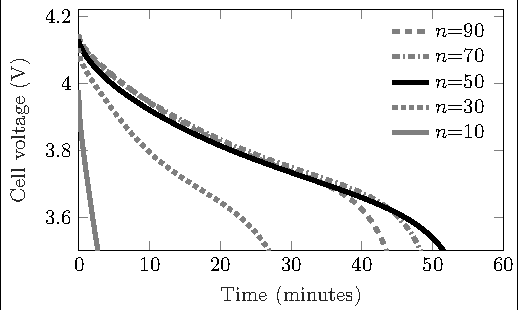
\includegraphics[trim=4 4 2 4,clip]{fig_CC_discharge_curves.pdf}
        \captionsetup{labelsep=note}
        \caption
        [%
        Voltage curves for a \SI{60}{\ampere} galvanostatic discharge from
        \SI{100}{\percent} \glsfmtshort{soc} until cut-off voltage for a few layer
        choices, in a pouch cell of fixed exterior height.
        ]%
        {%
            Terminal voltage curves of a Li-ion cell (with parameters
            given in \cref{tbl:lcoSimParamslayeropt}) under a \SI{60}{\ampere}
            galvanostatic discharge beginning from \SI{100}{\percent}
            \glsfmtshort{soc} until lower cut-off voltage for a few layer
            choices~$n$, in a pouch cell of fixed exterior height. The maximum
            usable energy is achieved for an intermediate choice of $n$
            that corresponds to neither the highest nominal capacity layer
            configuration ($n$=\num{10}) nor the highest electrode surface area
            configuration ($n$=\num{90}).
        }%
        \label{fig:fig_CC_discharge_curves}
        \mpfootnotes[1]
        \footnotetext{{The   rationale  behind  choosing   this  specific
                magnitude  of  applied  current  is   explained  in  the  section  dealing  with
        \hyperlink{refcellselection}{selection of a  suitable reference capacity cell} (also see \cref{sec:surfareaperlayer}).}}

        \footnote{This figure was created by \mbox{Ian Campbell} who asserts copyright,
            with intellectual contributions from and the right to use asserted by
        \mbox{Krishnakumar Gopalakrishnan}.}
    \end{minipage}
\end{figure}

As  seen  in \cref{fig:fig_CC_discharge_curves},  during  the  initial phase  of
discharge, the terminal voltage  of the cell is the highest  for the two highest
layer choices  \ie{} $n  = 90$  and $n=70$. Consistent  with the  explanation in
\cref{subsec:layeroptmotivation}, these  two layer choices have  thin electrodes
and hence  comparatively low resistances  leading to only a  small overpotential
drop within the cell. However, as expected, their total energy is lower than the
cell with  $n=50$ layers as  evidenced by  their relative run-times  until lower
cut-off voltage.  This is to  be expected as the  thin electrodes of  these high
layer-count cells cannot  store a large volume of active  material. Based on the
explanation  from \cref{subsec:layeroptmotivation},  it  is  expected that  this
trend will  continue \ie{} the  lower the layer  count, the higher  the run-time
until cut-off. If this were the case, prima facie it seems that the optimisation
task is trivial.

Inspecting the discharge curves of lower layer choices brings into limelight the
concept of \emph{usable} energy. Contrary  to expectations, the discharge curves
corresponding  to very  low layer  counts in  \cref{fig:fig_CC_discharge_curves}
terminate even earlier than $n=50$. This is  owing to the fact that although the
total  stored energy  in cells  with low  layer counts  is much  higher, only  a
fraction  of it  is  usable.  This aspects  introduces  non-convex dynamics  (as
discussed below) to an otherwise linear optimisation task.

For  instance,  when $n  =  10$,  the terminal  voltage  of  the cell  collapses
instantaneously, reaching cut-off  voltage whilst its \gls{soc}  remains as high
as \SI{96}{\percent}. At very low layer  counts, the thickness of each electrode
is high. This presents a high resistance  to the flow of charges thereby leading
to  high overpotential  drops  within the  cell. The  usable  energy under  this
\SI{60}{\ampere} galvanostatic  discharge for various layer  choices is compared
in \cref{tbl:CC_discharge_curves_table}. It can be  seen that for very low layer
counts,  the usable  energy that  can be  extracted is  miniscule, albeit  their
theoretical  capacity~$Q_n$  are  in-fact  the highest.  The  usable  energy  in
\SI{}{\watthour} reported in \cref{tbl:CC_discharge_curves_table} is obtained by
multiplying the integral  of the area under each discharge  curve by the applied
current \ie{}  \SI{60}{\ampere} with  the appropriate  scaling of  the time-base
(from minutes to hours).

% -*- root: ../../main.tex -*-
%!TEX root = ../../main.tex

\begin{table}[!htbp]
    \caption
    [%
    Theoretical  capacity \&  usable energy  of a  Li-ion cell  for a  few layer
    choices under a \SI{60}{\ampere} galvanostatic discharge
    ]
    {%
        Theoretical capacity and usable energy of a Li-ion cell (with parameters
        given in \cref{tbl:lcoSimParamslayeropt}) for  a few layer choices under
        a \SI{60}{\ampere} galvanostatic discharge.
    }%
    \label{tbl:CC_discharge_curves_table}
    \centering
    \begin{tabular}{@{} S[table-format=2.0] S[table-format=1.2] S[table-format=2.2]  S[table-format=3.2] S[table-format=2.2] @{}}
        \toprule
        \multicolumn{1}{@{} l}{$n$} &  \multicolumn{1}{c}{\footnotesize C-rate} & \multicolumn{1}{c}{\footnotesize \makecell{Theoretical \\ Capacity  (\si{Ah})}} & \multicolumn{1}{c}{\footnotesize \makecell{Usable \\ Energy \si{(Wh)}}} & \multicolumn{1}{c @{}}{\footnotesize \makecell{Remaining \\ SOC  (\si{\percent})}} \\
        \midrule
        90 & 1.24 & 48.25 & 166.46 & 9.84  \\
        70 & 1.11 & 53.99 & 184.80 & 10.26 \\
        50 & 1.00 & 59.73 & 195.47 & 13.51 \\
        30 & 0.92 & 65.47 & 101.20 & 58.95 \\
        10 & 0.84 & 71.21 & 10.15  & 96.22 \\
        \bottomrule
    \end{tabular}
\end{table}


\Cref{tbl:CC_discharge_curves_table}  also brings  into view  the fact  that the
\mbox{C-rate} of the  cell becomes a variable quantity even  for a galvanostatic
discharge,  due to  the dependence  of  its nominal  capacity on  the number  of
layers~$n$.  This  represents  a  departure  from  the  norm  in  the  modelling
community, wherein the performance of cells  are quantified as a function of the
applied C-rate \eg{}  in \cref{ch:spmanalysis} and \cref{ch:newelectrolytemodel}
of this  thesis. However,  this preliminary  investigation has  quickly revealed
that this normalised  quantity does not hold much importance  in any study where
the number of layers within a pouch cell is varied.

Taking into account  these factors, a reasonable choice of  the number of layers
in  this specific  \SI{60}{\ampere} galvanostatic  application for  this example
cell  could  be $n=50$.  This  represents  a  practical compromise  between  the
surface area  available for  reaction and  the total  volume of  active material
accommodated.  This layer  selection offers  the highest  usable energy  for the
given discharge rate, out of the finite layer configurations considered.

In this  sample study, only  a handful of  layer choices were  considered, which
represents  only  a  small  possibility  of  the  overall  design  space  to  be
considered. Furthermore,  thermal considerations were  not explored so  far. For
robust  cell design,  manufacturers  shall need  a  widely applicable  model-led
design tool that  can tackle the wide-ranging possible scenarios  that can occur
in real-life operating conditions. A deterministic set of optimality criteria is
also to  be formulated. The choice  $n=50$, therefore does not  represent in any
way the general  optimal layer choice even for this  example cell. However, this
serves as an illustrative demonstration of the trade-offs in energy versus power
handling capability of a cell for  a specific set of conditions. Furthermore, it
introduces the  complicating aspect of  \emph{useable} capacity into  what would
have  otherwise been  a  trivial  exercise, thereby  setting  the  tone for  the
development of a general layer optimisation framework for pouch cells.

